\documentclass[12pt]{article}

\usepackage[utf8]{inputenc}
\usepackage[T1]{fontenc}

% clickable links in pdf
\usepackage{hyperref}

% make title variable available
\usepackage{titling}

% create own header footer
\usepackage{fancyhdr}

% images
\usepackage{graphicx}

% grafics powerfull and hard
\usepackage{tikz}

% character spacing to fill line
\usepackage{microtype}

% image placement with [H]
\usepackage{float}

% fancy quotes
\usepackage{epigraph}

% extra symbols
\usepackage{textcomp}

% display code
\usepackage{listings}

% icons
\usepackage{fontawesome}

% set dimmensions of page
\usepackage[footskip=80pt, headheight=15pt]{geometry}

% tables
\usepackage{tabularx}
\usepackage{makecell}

% make code copyable
\lstset{
	upquote=true,
	columns=fullflexible,
	literate={*}{{\char42}}1
	{-}{{\char45}}1
}

\newsavebox{\picbox}

\graphicspath{ {./images/} }

% command for rounded corners
\newcommand{\cutpic}[3]{
	\savebox{\picbox}{\includegraphics[width=#2]{#3}}
	\tikz\node [draw, rounded corners=#1, line width=4pt,
	color=white, minimum width=\wd\picbox,
	minimum height=\ht\picbox, path picture={
		\node at (path picture bounding box.center) {
			\usebox{\picbox}};
	}] {};}

\title{
	\Huge
	\textbf{Globalizer} \\
	\vspace{0.2cm}
	\LARGE
	Detailkonzpet
}

\date{18.10.2018}

\author{
	Koller, Jonas\\
	\texttt{jonas.koller@gmx.ch} \\
	Wolfisberg, Donato \\
	\texttt{donato.wolfisberg@gmail.com}
}

\pagestyle{fancy}
\fancyhf{}
\lhead{BBZW Sursee Rötheli Manfred}
\rhead{Globalizer Detailkonzept}
\lfoot{Jonas Koller \& \\ Donato Wolfisberg}
\cfoot{\thedate}
\rfoot{\thepage}

\renewcommand{\headrulewidth}{1pt}
\renewcommand{\footrulewidth}{1pt}

\renewcommand{\contentsname}{Inhalt}

\begin{document}
	\begin{titlepage}
		\pagenumbering{gobble}
		
		\begin{center}
			\vspace*{-2cm}
			\cutpic{0.8cm}{4cm}{logo.jpg}
			
			\thetitle
			
			\vspace{2cm}
			
			\textbf{\theauthor}
			
			\vspace{1.5cm}
			
			\thedate
		\end{center}
		
		\vfill
		
		\begin{figure}[H]
			\makebox[\linewidth]{
				
\includegraphics[width=1.3\linewidth]{globe.jpg}
			}
			\vspace*{-5cm}
		\end{figure}
	\end{titlepage}
	
	\newpage
	\pagenumbering{Roman}
	
	\begin{center}
		\makebox[\textwidth]{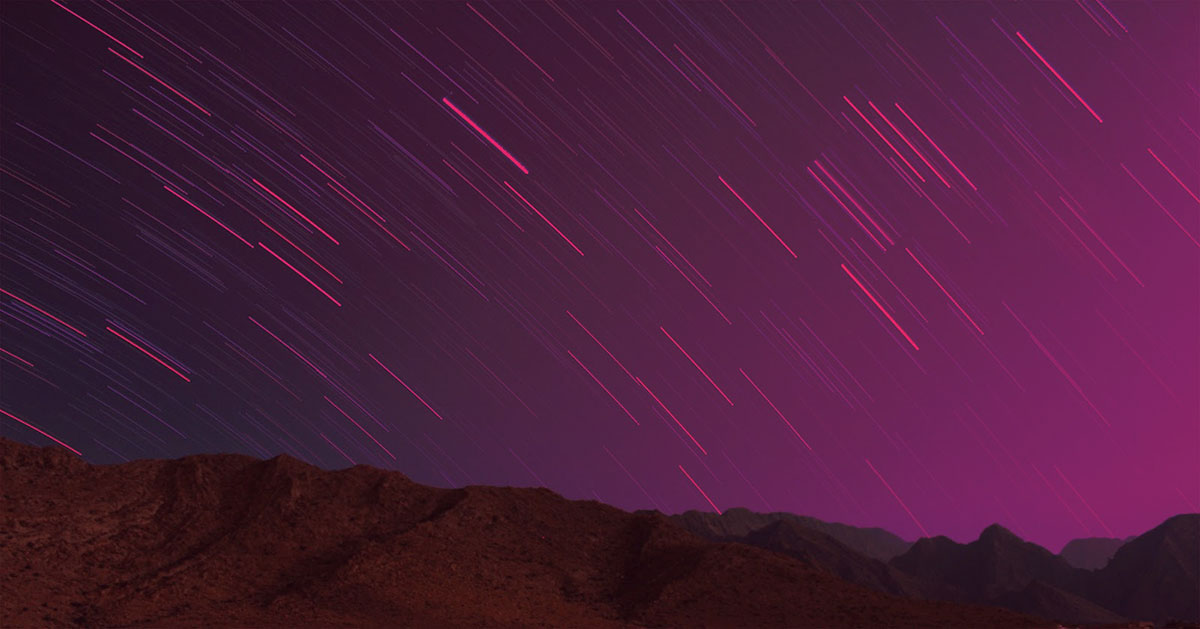
\includegraphics[width=\paperwidth]{nightsky.jpg}}
	\end{center}
	
	\section{Einleitung}
	Dieses Dokument behandelt das Detailkonzept des Projekts Globalizer. Ziel und Zweck des Dokuments ist es, die fachlichen Anforderungen technisch zu umschreiben, damit diese später implementiert werden können. Zudem soll das Gesamtbild unserer Applikation klar gemacht werden und die Komponenten, sowie der Datenaustausch genau beschrieben werden. Es werden auch all unsere Technologieentscheide vermerkt und begründet. Zusammengefasst soll dieses Dokument also eine klare, wie auch detailierte Übersicht zu den technischen Aspekten unseres Projekts sein.
	
	\newpage
	
	\section{Allgemeine Informationen}
	Hier folgt eine kurze Auflistung der Informationen zu diesem Dokument, dem Ent\-wicklungsteam und dem aktuellen Stand.
	
	\subsection{Projektmitarbeiter}
	\begin{table}[h]
		\begin{tabularx}{\textwidth}{|l|l|X|l|}
			\hline
			\textbf{Name} & \textbf{Vorname}  & \textbf{E-Mail}                & \textbf{Funktion}     \\ \hline
			Koller        & Jonas             & jonas.koller@gmx.ch            & Projektleiter         \\ \hline
			Wolfisberg    & Donato            & donato.wolfisberg@gmail.com    & Entwickler            \\ \hline
			Gian          & Ott               & gian\_ott@sluz.ch              & Prüfer                \\ \hline
			Manuel        & Troxler           & manuel\_troxler@sluz.ch        & Prüfer                \\ \hline
		\end{tabularx}%
	\end{table}
	
	\subsection{Änderungskontrolle}
	\begin{table}[h]
		\begin{tabularx}{\textwidth}{|l|l|l|X|}
			\hline
			\textbf{Version} & \textbf{Datum} & \textbf{Ausführende Stelle} & \textbf{Bemerkung}                     \\ \hline
			1                & 21.09.2018     & Projektteam                 & \makecell[l]{Erste Version des Dokuments \\ erstellt}  \\
			2                & 23.09.2018     & Projektteam                 & \makecell[l]{Gesamtüberblick erstellt}  \\
			3                & 25.09.2018     & Projektteam                 & \makecell[l]{Zielkatalog erstellt}  \\
			4                & 27.09.2018     & Projektteam                 & \makecell[l]{Abschliessende Arbeiten}  \\
			\hline
		\end{tabularx}
	\end{table}
	
	\subsection{Prüfung}
	\begin{table}[h]
		\begin{tabularx}{\textwidth}{|l|l|X|}
			\hline
			\textbf{Version} & \textbf{Datum} & \textbf{Ausführende Stelle}     \\ \hline
			4                 & 27.09.2018    & Gian Ott                        \\ \hline
		\end{tabularx}
	\end{table}
	
	\newpage
	\tableofcontents
	\newpage
	
	\pagenumbering{arabic}
	
	
	\section{Systemkomponenten}
	Das Projekt verwendet einen klassische Client - Server Architektur. Somit ergeben sich bei uns drei Hauptkomponenten. Dies ist das Backend, das Frontend und die Datenbank. Wir werden folgend beschreiben, wie diese genau aufgebaut sind.
	\subsection{Frontend}
	In der Fontend-Komponente soll die Schnittstelle zwischen Endbenutzer und Backend-System implementiert werden. Wir werden dies mit einer Weboberfläche machen. Diese Komponente soll unabhängig vom Backend-System auf einem CDN gehostet werden können. Diese Masnahme verringert die Wartenzeiten des Endnutzers deutlich.
	\subsection{Backend}
	Unser Backend-System soll die Schnittstelle zwischen den Daten und dem Frontend abbilden. Hier werden die rohen Daten von der Datenbank aufbereitet, berechnungen durchgeführt und die Security-Aspekte grösstenteils abgedeckt. Die Authentifizierung, Autorisierung und Überprüfung der übermittelten Daten soll hier stattfinden. Das Backend soll möglichst klein gehalten werden, damit der Wartungsaufwand minimal bleibt. Es soll so gebaut werden, dass es gut skalierbar verwendet werden kann. Aspekte wie Load-Balancing und Upscaling sollen vom Hoster übernommen werden.
	\subsection{Datenbank}
	Die Datenbank bildet den dritten Teil unseres Systems. Hier soll eine InMemory-Datenbank verwendet werden. Diese brauch weniger Leistung und sorgt für zusätzliche Geschwindigkeit beim System. Uns ist bewusst, dass die Datenbank ihren aktuellen Stand bei einem Systemabsturz verlieren kann. Da es sich jedoch um einen flüchtigen Chat handelt, welcher nicht zu 100\% sicher persistiert werden muss, kann eine InMemory-DB verwendet werden.
	
	\newpage
	
	\subsection{Zonen-Übersicht}
	Auf der nachfolgenden Grafik kann unsere Architektur im groben ausgelesen werden. Das System ist in die drei "Komponenten-Zonen" unterteilt. Diese sollen wenn möglich unabhängig von den anderen deploybar sein. Dies ermöglicht es uns später auch, unsere Deployment-Zyklen zu vereinfachen. Im Backend-System ist zusätzlich auch der LoadBalancer eingezeichnet, welcher vom Hoster übernommen wird.\newline
	
	\noindent
	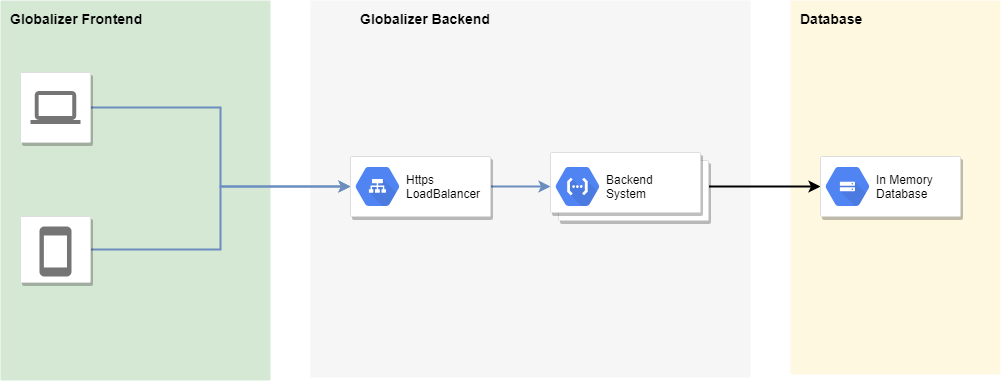
\includegraphics[width=\linewidth]{system-components.png}
	
	\section{Design-Pattern}
	Da werder unser Backend, noch unser Frontend objektoriertiert ist, können keine Klassendiagramme erstellt werden. OOP-Eigenschaften wie Vererbungen und beziehungen werden bei diesem Projekt auch kaum benutzt. Aus diesem Grund verzichten wir auf diese Diagramme. Wir verwenden anstelle dessen aber ein UML-Aktivitätsdiagramm, um unsere Abläufe zu visualisieren.
	
	\subsection{Architektur Backend}
	Das Backend wird in NodeJS erstellt. Es nutzt Websockets zur Kommunikation mit dem Frontend. Das Websocket-Protokoll ist auf TCP basiert und erlaubt bidirektionale Verbindungen zwischen Server und Client. Das Backend ist offen für neue Verbindungen. Wenn sich ein neuer Benutzer anmeldet, registriert dieser sich beim Backend. Dieses hört danach auf Anfragen des Frontends. Im gegenzug sendet das Backend neue Nachrichten selbst an das Frontend. Durch dieses "Bidirectional Message Pattern" können wir einiges an Bandbreite einsparen, da wir nicht immer wieder Fetch-Anfragen senden müssen um den Client auf dem aktuellen Stand zu behalten. Wir konnten somit das "Fetch"-Antipattern umgehen, da dieses für eine Chat-Applikation ungeeignet ist. In der folgenden Grafik kann ausgelesen werden, wie die der Ablauf bei Anfragen an den Server aussehen.
	
	\section{Analyse des IST-Systems}
	Im Moment wird die Kommunikation zwischen den Schülern und den Lehrern über diverse Kanäle geführt: Mail, Telefon, Whatsapp und weitere. Die neue Applikation kann diese Kanäle nicht ersetzen, sondern im Bereich des Chats die Austausch von Informationen auf anonymer Basis ermöglichen.
	
	\subsection{Zielsetzungen}
	\subsubsection{Muss-Ziele}
	\begin{enumerate}
		\item \faGlobe~   Globaler Gruppen Chat
		\item \faUser~    Hinterlegen eines Benutzernamens
		\item \faKey~     Benutzer muss den Chat später wieder aufnehmen können. z.B. Cookies oder Session Storage
		\item \faMobile~  Die Seite für Mobile geräte optimieren
	\end{enumerate}
	
	\subsubsection{Kann-Ziele}
	\begin{enumerate}
		\item \faUsers~   Private Chats zwischen zwei Personen
		\item \faGoogle~  Authentifizierung über Google Accounts, aber trotzdem anonym
	\end{enumerate}
\end{document}
